\chapter{SCRUM Proces}
\label{chapter:scrum}
Dette kapitel vil beskrive \emph{SCRUM}-processen, hvilke modifikationer der blev foretaget samt analysen bag og hvordan det blev anvendt til at strukturere projektet. 
I \Cref{chapter:conclusion} forefindes afsnittet \Cref{sec:conclusion_summary}, der opsummerer \emph{SCRUM}-processen og dens anvendelse i projektet.
Alle \emph{User Stories} er at finde i bilag \Cref{appendix:userstories}.

\section{Workflows}
Workflows er normalt ikke en del af \emph{SCRUM}-processen men en metode, hvorpå jeg kunne tage noget, der var i størrelsen af en \emph{epic user story} og dele den op i mindre \emph{User Stories}. 
Jeg har valgt at bruge denne metode, da den låner elementer fra \emph{Persona}-tilgangen, men i et format, der gør det mere håndgribeligt at omsætte til \emph{User Stories}.
Samtidig giver det et fokus på funktionalitet for slutbrugeren og det design, der skal støtte op om det.

\subsection{Workflow eksempel}
Situation: Medarbejder (blomsterdekoratør) ekspederer en ordre.
Formål: At håndtere indkommende ordrer og forberede blomsterarrangementer.
\begin{enumerate}
    \item Medarbejder logger ind på ordreportalen.
    \item Medarbejder gennemser listen over dagens ordrer og vælger en ordre til ekspedition.
    \item Medarbejder forbereder blomsterarrangementet i henhold til kundens specifikationer.
    \item Medarbejder markerer ordren som 'klar til levering' eller 'klar til afhentning'.
    \item Medarbejder opdaterer ordrestatus i systemet.
    \label{item:workflow-eksempel}
\end{enumerate}

\begin{figure}[H]
    \centering
    \begin{minipage}[b]{0.45\textwidth}
        \centering
        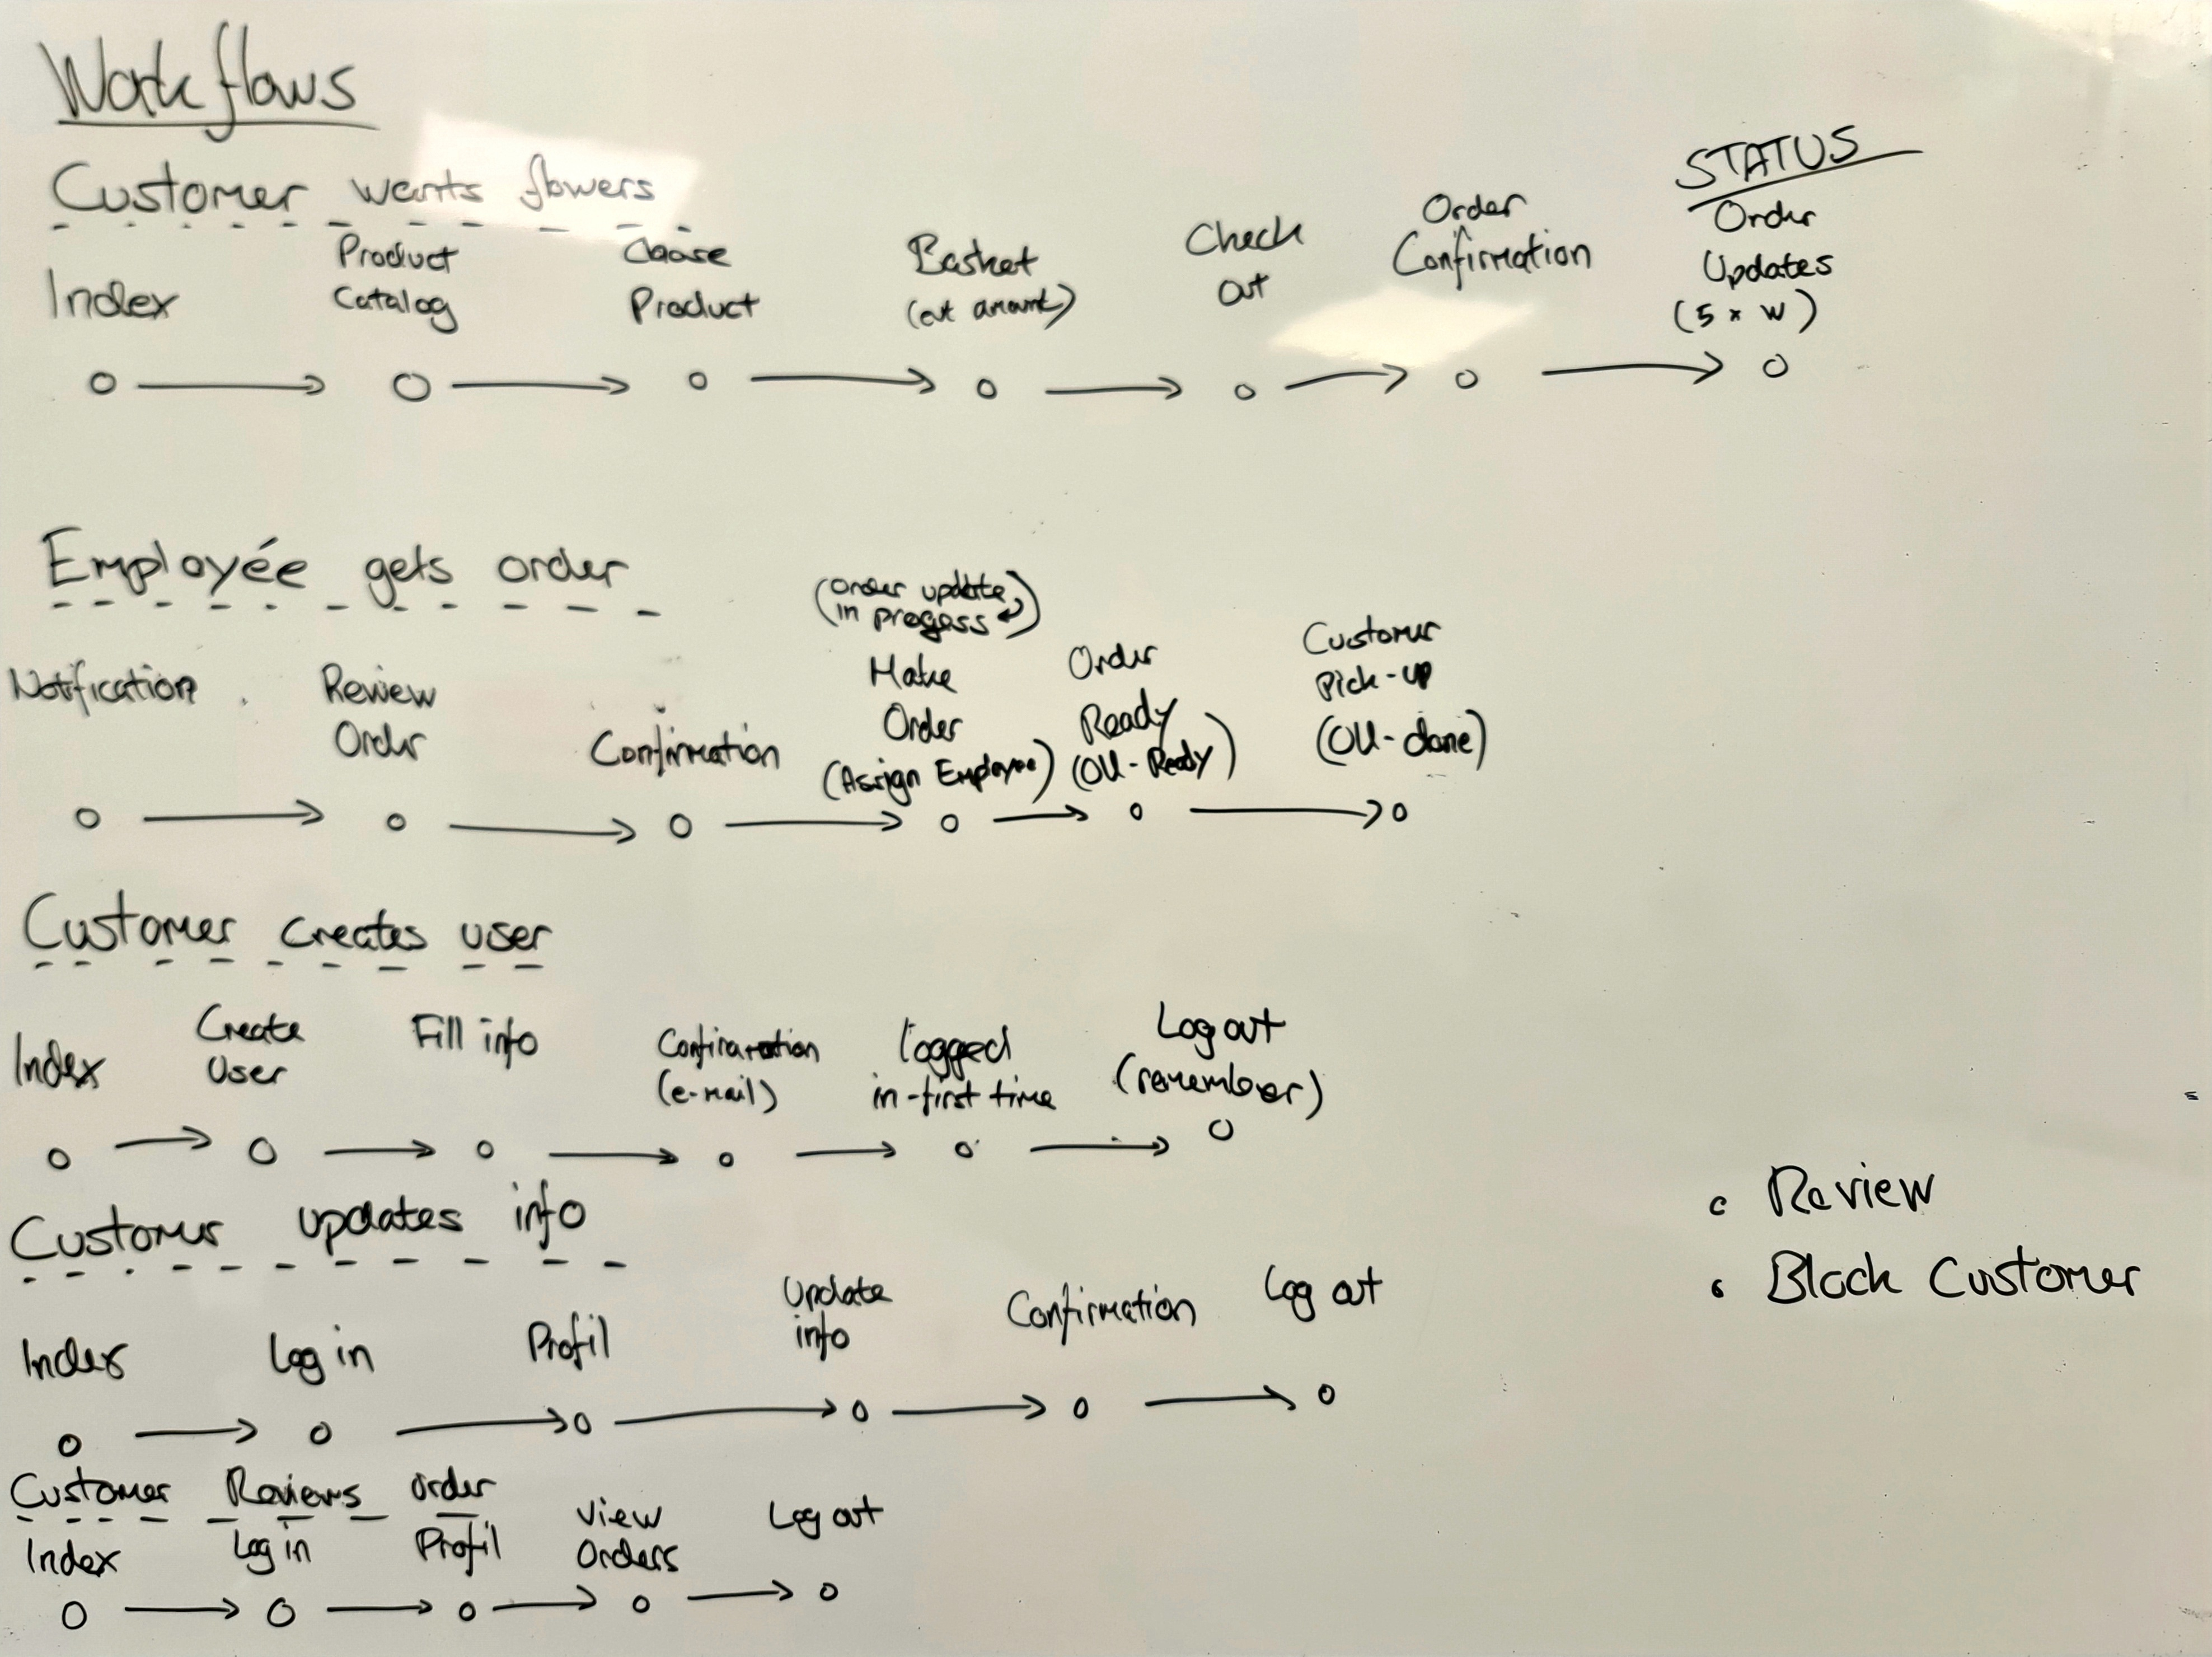
\includegraphics[width=\textwidth]{figures/scrum/workflow-board1.jpg}
        \caption{Workflow Board 1}
        \label{fig:workflow-board1}
    \end{minipage}
    \hfill
    \begin{minipage}[b]{0.45\textwidth}
        \centering
        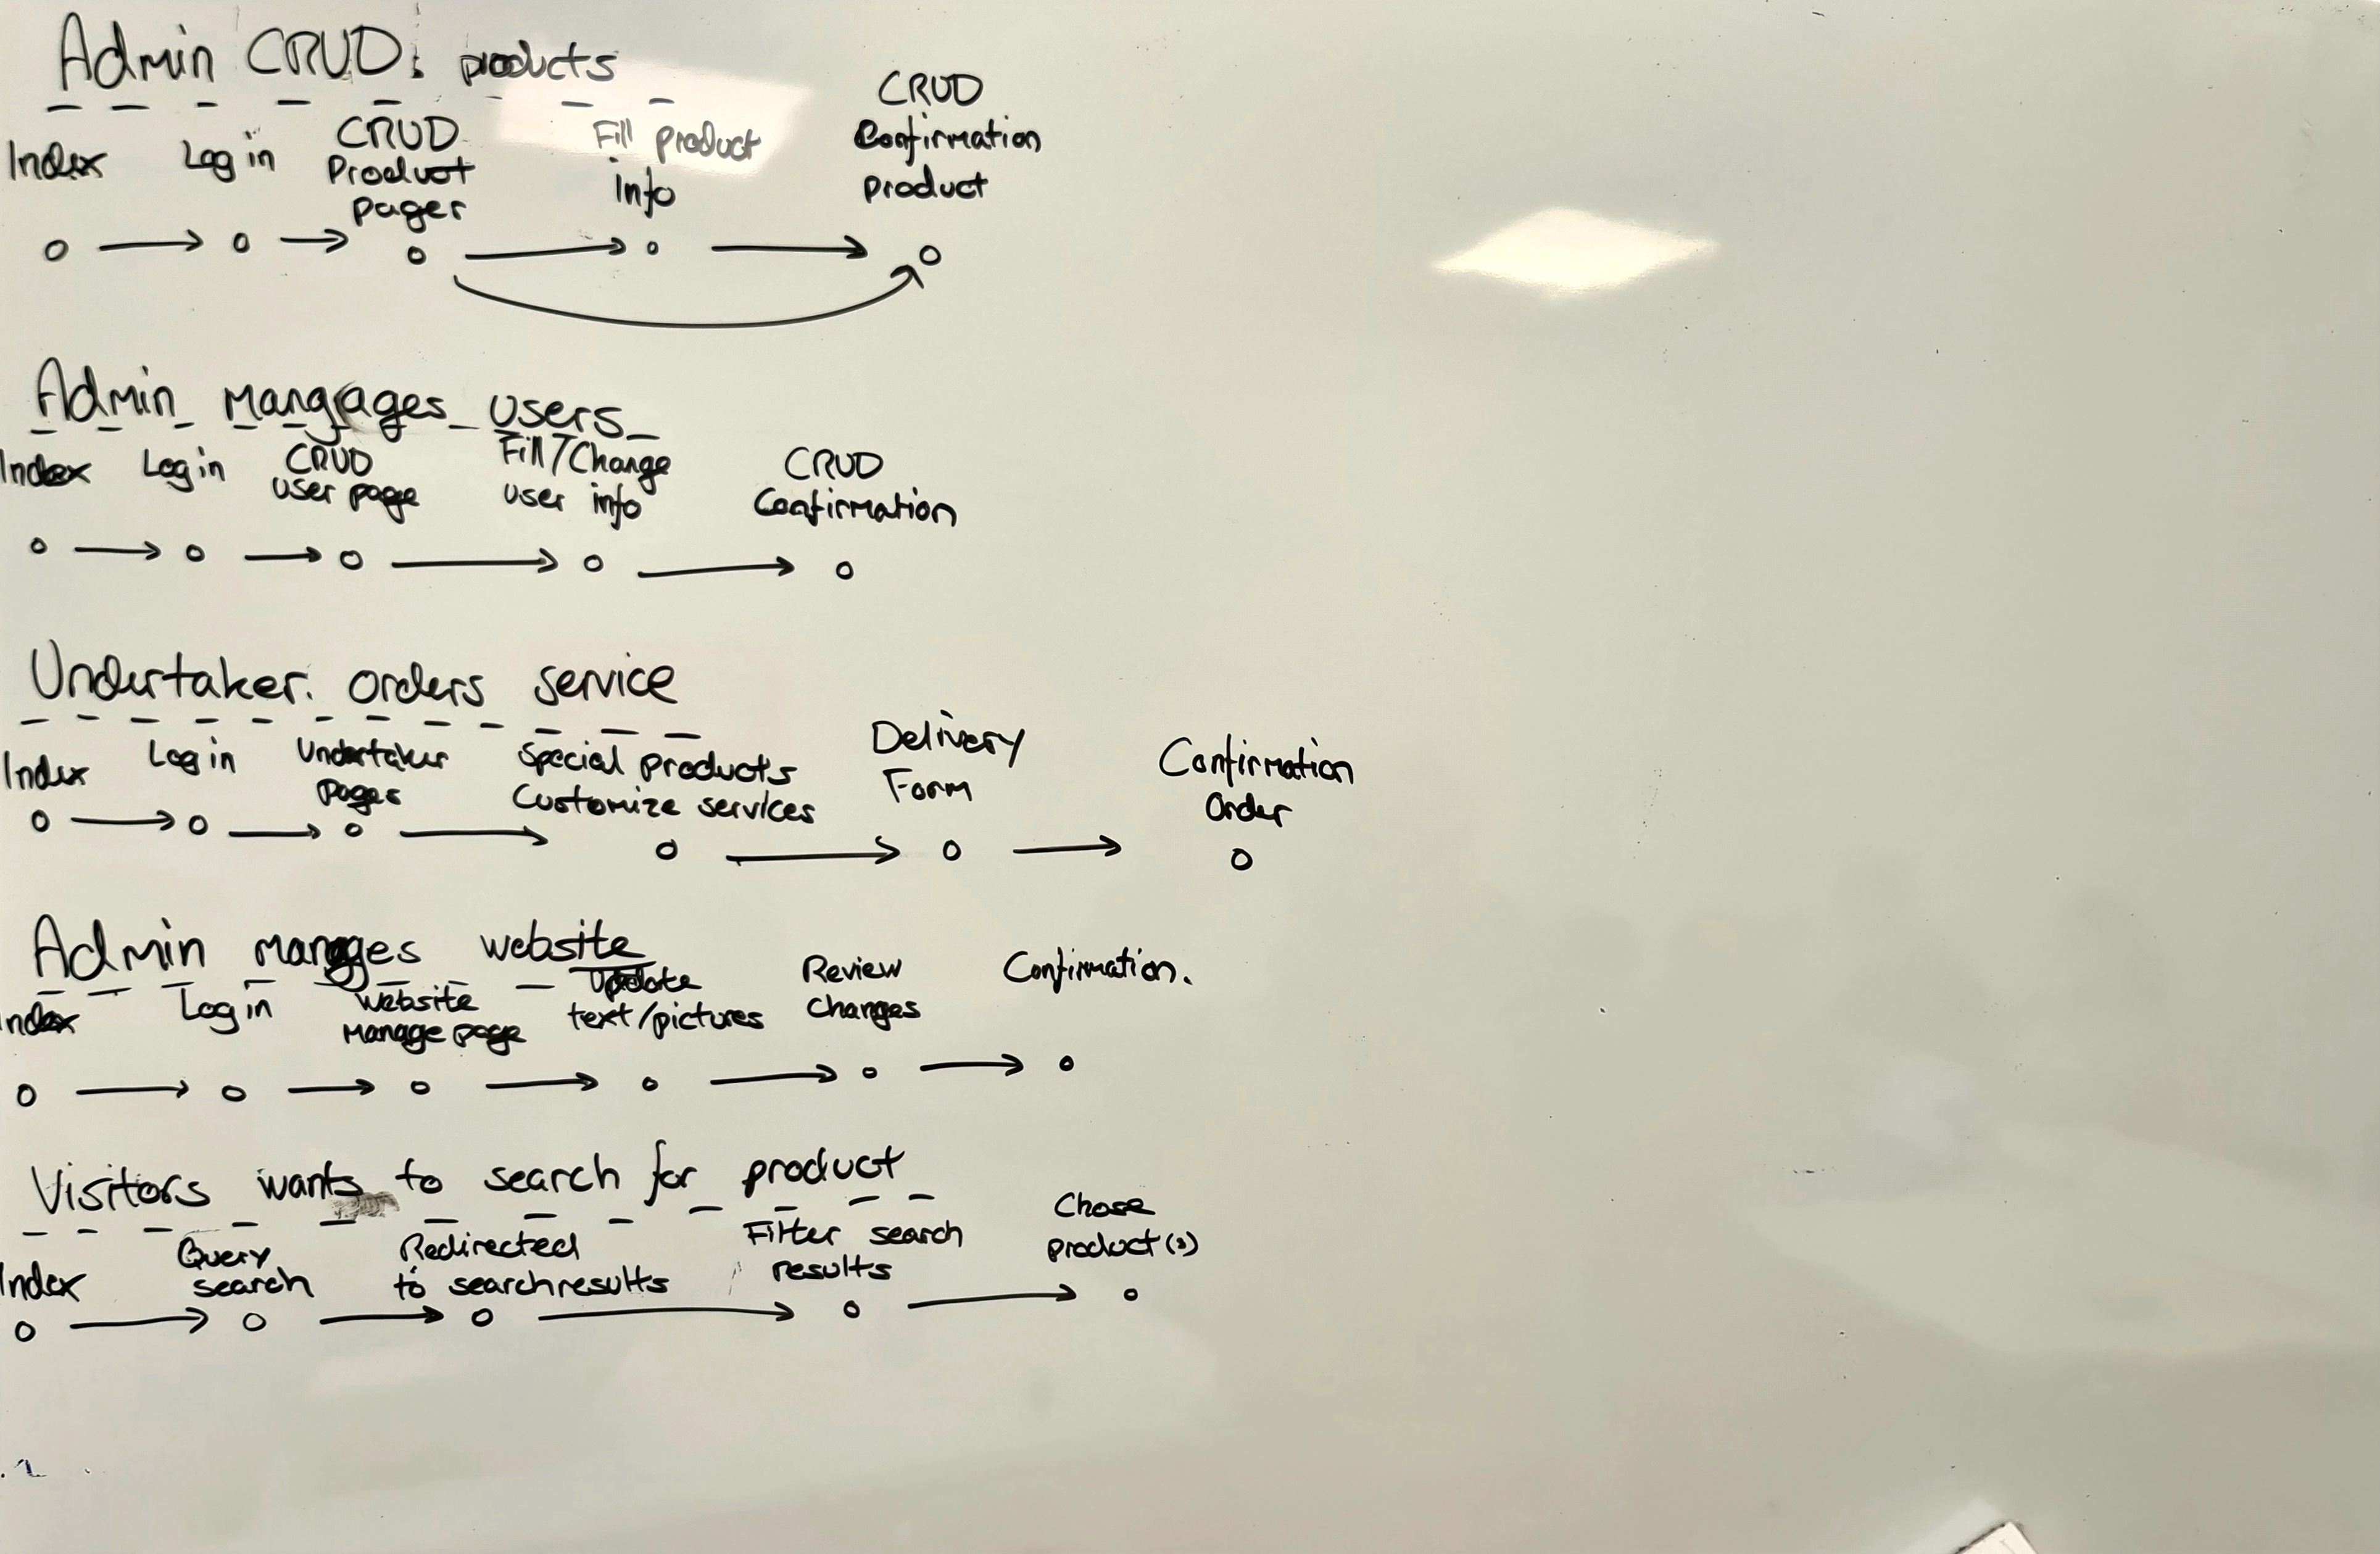
\includegraphics[width=\textwidth]{figures/scrum/workflow-board2.jpg}
        \caption{Workflow Board 2}
        \label{fig:workflow-board2}
    \end{minipage}
\end{figure}

Rent fysisk blev de opskrevne Workflows sat op på en whiteboard. Herefter blev der sat ringe om områder, der kunne omsættes til \emph{User Stories}.
Workflow-punkter, der gik igen eller ville afføde den samme funktionalitet, blev overstreget og samlet i en \emph{User Story}.
I eksemplet fra \Cref{item:workflow-eksempel} kunne det være følgende \emph{User Stories}:
\begin{enumerate}
    \item "Som medarbejder vil jeg kunne logge ind på ordreportalen, så jeg kan ekspedere ordrer."
    \item "Som medarbejder vil jeg kunne se ordredetaljer om blomsterarrangementet, så jeg kan ekspedere ordrer."
    \item "Som medarbejder vil jeg kunne opdatere ordrestatus, så jeg kan tydeliggøre for alle brugere, hvor langt ordren er."
    \label{item:workflow-us-eksempel}
\end{enumerate}

\begin{figure}[H]
    \centering
    \begin{minipage}[b]{0.45\textwidth}
        \centering
        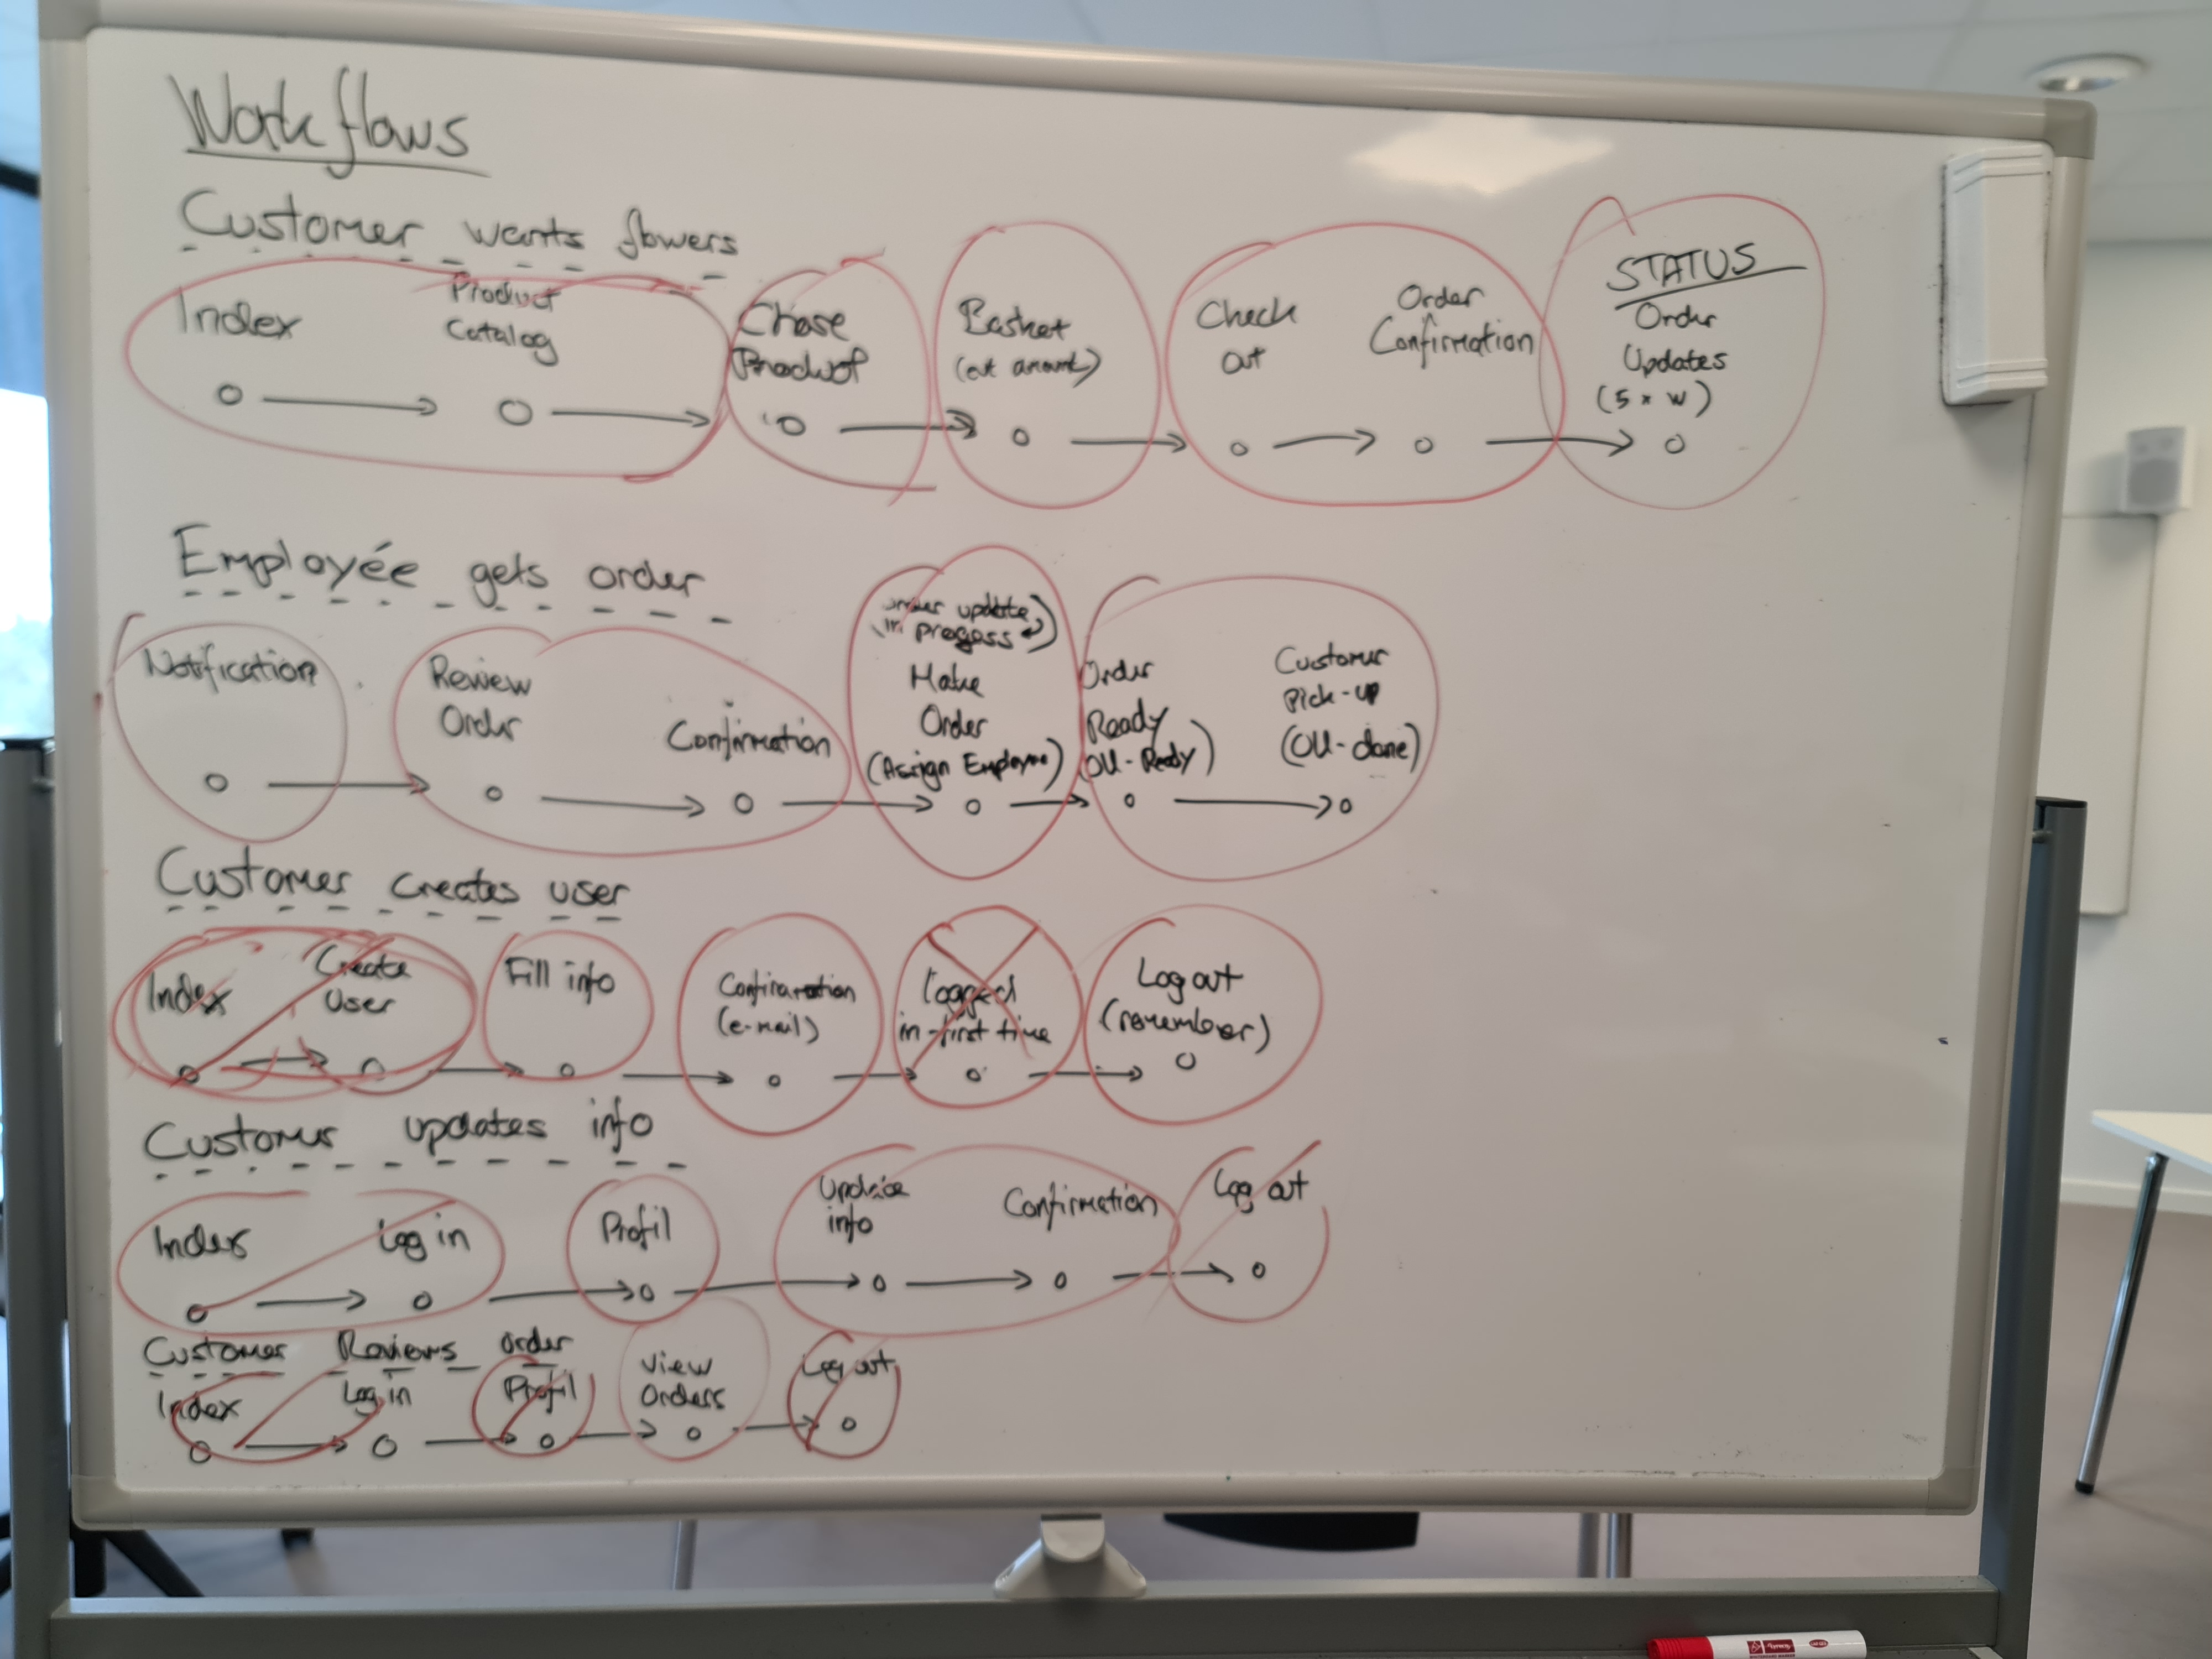
\includegraphics[width=\textwidth]{figures/scrum/workflow-board-red-rings1.jpg}
        \caption{Workflow Board 1}
        \label{fig:workflow-board-red-ring1}
    \end{minipage}
    \hfill
    \begin{minipage}[b]{0.45\textwidth}
        \centering
        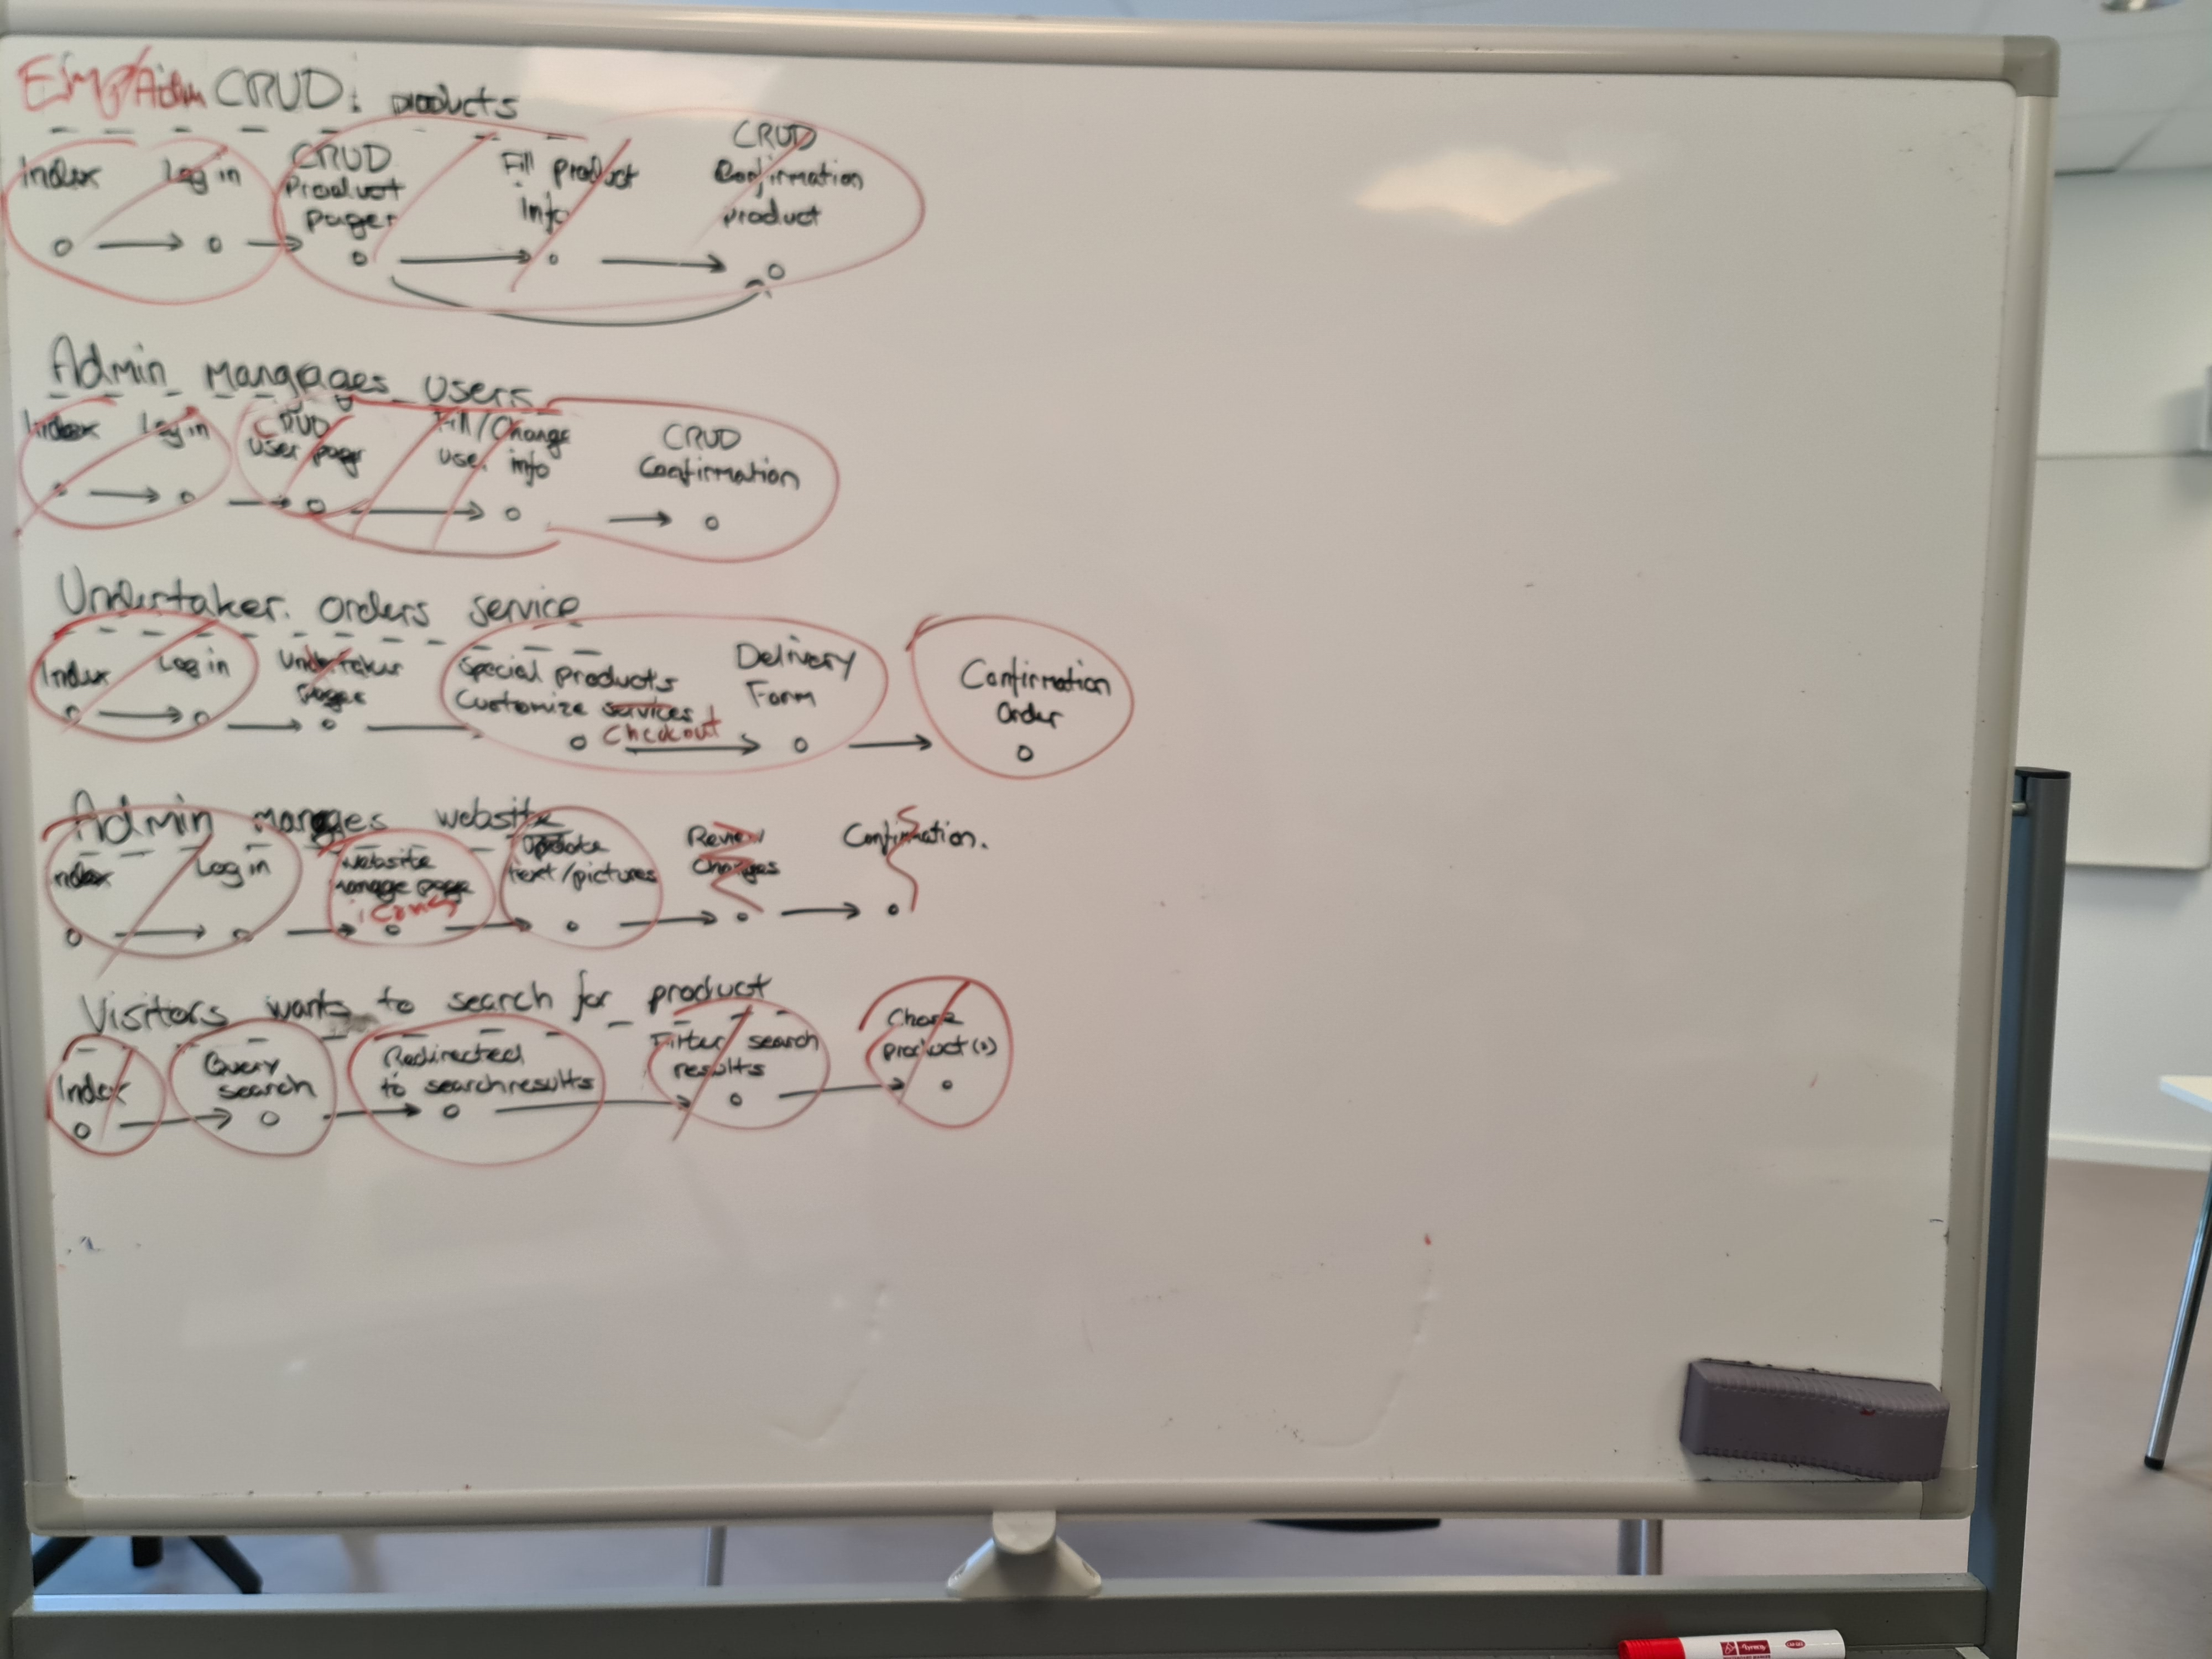
\includegraphics[width=\textwidth]{figures/scrum/workflow-board-red-rings2.jpg}
        \caption{Workflow Board 2}
        \label{fig:workflow-board-red-ring2}
    \end{minipage}
\end{figure}

Dette er stadig relativt store \emph{User Stories}. Ved at tilknytte \emph{Tasks} til hver \emph{User Story}, bliver de mere overskuelige og 
nemmere at tildele \emph{Acceptance Criteria}. Dermed får man et godt overblik over, hvad der skal til for at implementere funktionaliteten.

\section{User Stories}
Der blev skrevet \emph{User Stories} for kunder (underforstået private), bedemænd, medarbejdere og bestyrer, da de har forskellige behov og derfor også forskellige \emph{User Stories}.
Da hensigten med \emph{User Stories} er at beskrive funktionalitet fra slutbrugerens perspektiv, vil nogle elementer overlappe. Det kan f.eks. være, at både en medarbejder og en kunde kunne logge ind på webshoppen.
I sådanne tilfælde blev der skrevet en \emph{User Story} for hver, hvis de havde forskellige behov og derfor også forskellige \emph{Acceptance Criteria}.
Ved for stort overlap blev de slået sammen til en \emph{User Story}, der dækkede begge brugere.

\subsection{Opbygning af User Stories}
\emph{User Stories} blev skrevet i formatet "Som [rolle] ønsker jeg [handling], med det formål [resultat]".
Dette format sikrer, at \emph{User Stories} er fokuseret på funktionalitet og ikke teknologi.
Derudover blev der tilføjet \emph{Tasks} for at give klarhed til udvikleren om, hvad der konkret skulle gøres, samt \emph{Acceptance Criteria} for at sikre, at \emph{User Stories} var klare og præcise.

\subsection{Prioritering af User Stories}
\emph{User Stories} blev indledende prioriteret efter \emph{MoSCoW}-metoden, hvor de blev inddelt i fire kategorier: Must have, Should have, Could have og Won't have.
Det var dog ikke givende, da scope allerede var blevet afgrænset. Derfor blev \emph{User Stories} prioriteret efter, hvad der var vigtigst for slutbrugeren og med henblik på, at der hurtigt skulle kunne leveres en funktionel kerne af produktet.
\emph{User Stories} uden for scope forblev som "gode ideer" i \emph{product backloggen}.

\subsection{Estimering af User Stories}
\emph{User Stories} blev indledende estimeret i \emph{T-shirt sizes} efter XS, S, M, L, XL. Dette blev gjort for at fjerne fokus fra en numerisk værdi og i stedet fokusere på, hvor kompleks en \emph{User Story} var.
Estimeringen endte med at anvende \emph{Story Points} efter Fibonacci-sekvensen 1, 2, 3, 5 og 8. Dette skift skete, da det var nemmere at anvende tal, når bl.a. \emph{velocity} skulle beregnes.
Estimeringen tog udgangspunkt i tre faktorer:
\begin{itemize}
    \item Kodemængde, da overskuelighed forsvinder i takt med, at koden vokser, så risikoen for fejl stiger, og hvor lang tid debugging vil tage øges.
    \item Kodekompleksitet, baseret bl.a. på hvorvidt der skulle anvendes (mange) komplekse datatyper, eksotiske libraries som f.eks. \emph{httpContext}, eller der var mange afhængigheder.
    \item Funktionalitetskompleksitet, forstået som et holistisk skøn på, hvor mange delelementer denne feature ville gribe ind i, men bl.a. også hvor mange \emph{guardrails}, der skulle tilføjes for at sikre, at funktionaliteten virkede som forventet.
\end{itemize}
\emph{Planning Poker} blev anvendt i det gamle team til at estimere \emph{User Stories}. Hensigten var, at det skulle sikre, at alle i teamet havde en stemme, og at der blev taget højde for alle synspunkter.
Dette virkede redundant i det nye team, da der kun var én udvikler, der skulle estimere.

\subsection{User Story Mapping}
\emph{User Story Mapping} er en metode til at prioritere \emph{User Stories} og få et overblik over, hvad der skal implementeres først.
Det er en metode, der tager udgangspunkt i slutbrugerens behov og dermed sikrer, at de vigtigste funktionaliteter bliver implementeret først.
Her hjalp Workflows også med at identificere \emph{User Stories}, der kunne grupperes og prioriteres, fordi de netop beskrev en holistisk proces.
I eksemplet fra \Cref{item:user-story-mapping-eksempel} kunne det være, at \emph{User Stories} 1, 2, 3, 4 og 9 skulle implementeres først, da de dækker overordnede funktionaliteter, der er vigtige for kunden.

\subsection{User Story Mapping eksempel}
Kunden ønsker at kunne logge ind og se sine ordrer og betalinger. Dette kræver, at kunden kan logge ind, se en oversigt over sine ordrer, se en oversigt over sine betalinger og se detaljer om en ordre.
\begin{enumerate}
    \item "Som kunde vil jeg kunne logge ind, så jeg kan se mine ordrer og betalinger."
    \item "Som kunde vil jeg kunne se en oversigt over mine ordrer, så jeg kan følge med i, hvor langt de er."
    \item "Som kunde vil jeg kunne se en oversigt over mine betalinger, så jeg kan se, hvad jeg har betalt."
    \item "Som kunde vil jeg .. etc..."
    %\item "Som kunde vil jeg kunne se detaljer om en ordre, så jeg kan se, hvad jeg har betalt for."
    %\item "Som kunde vil jeg kunne se en oversigt over mine personlige oplysninger, så jeg kan se, hvad I har registreret om mig."
    %\item "Som kunde vil jeg kunne se detaljer om mine personlige oplysninger, så jeg kan se, hvad I har registreret om mig."
    %\item "Som kunde vil jeg kunne ændre mine personlige oplysninger, så jeg kan sikre, at de er korrekte."
    %\item "Som kunde vil jeg kunne slette mine personlige oplysninger, så jeg kan sikre, at de ikke længere er tilgængelige."
    %\item "Som kunde vil jeg kunne logge ud, så jeg kan sikre, at mine oplysninger ikke er tilgængelige for andre."
    \label{item:user-story-mapping-eksempel}
\end{enumerate}

\subsection{Product backlog}
Da tidsrammen for projektet var begrænset, blev der oprettet en \emph{Product Backlog}, der indeholdt alle \emph{User Stories}. Derfra blev der dog lavet en iterativ \emph{Sprint Planning} for hele projektet for at sikre, at scope for projektet var realistisk.
Alle \emph{User Stories} blev prioriteret og estimeret samt fordelt i de fem \emph{Sprints} i en prioriteret rækkefølge med de vigtigste på toppen, se figur \Cref{fig:trello-sprint-backlogs}. 
Dette skabte overblik over, hvad der skulle implementeres først, samt satte en indsats/belastning, både på \emph{Sprint} basis men også for hele projektet.
Dermed kunne det bruges som et styringsredskab til at sikre, at projektet blev færdigt til tiden.
\begin{figure}[H]
    \centering
    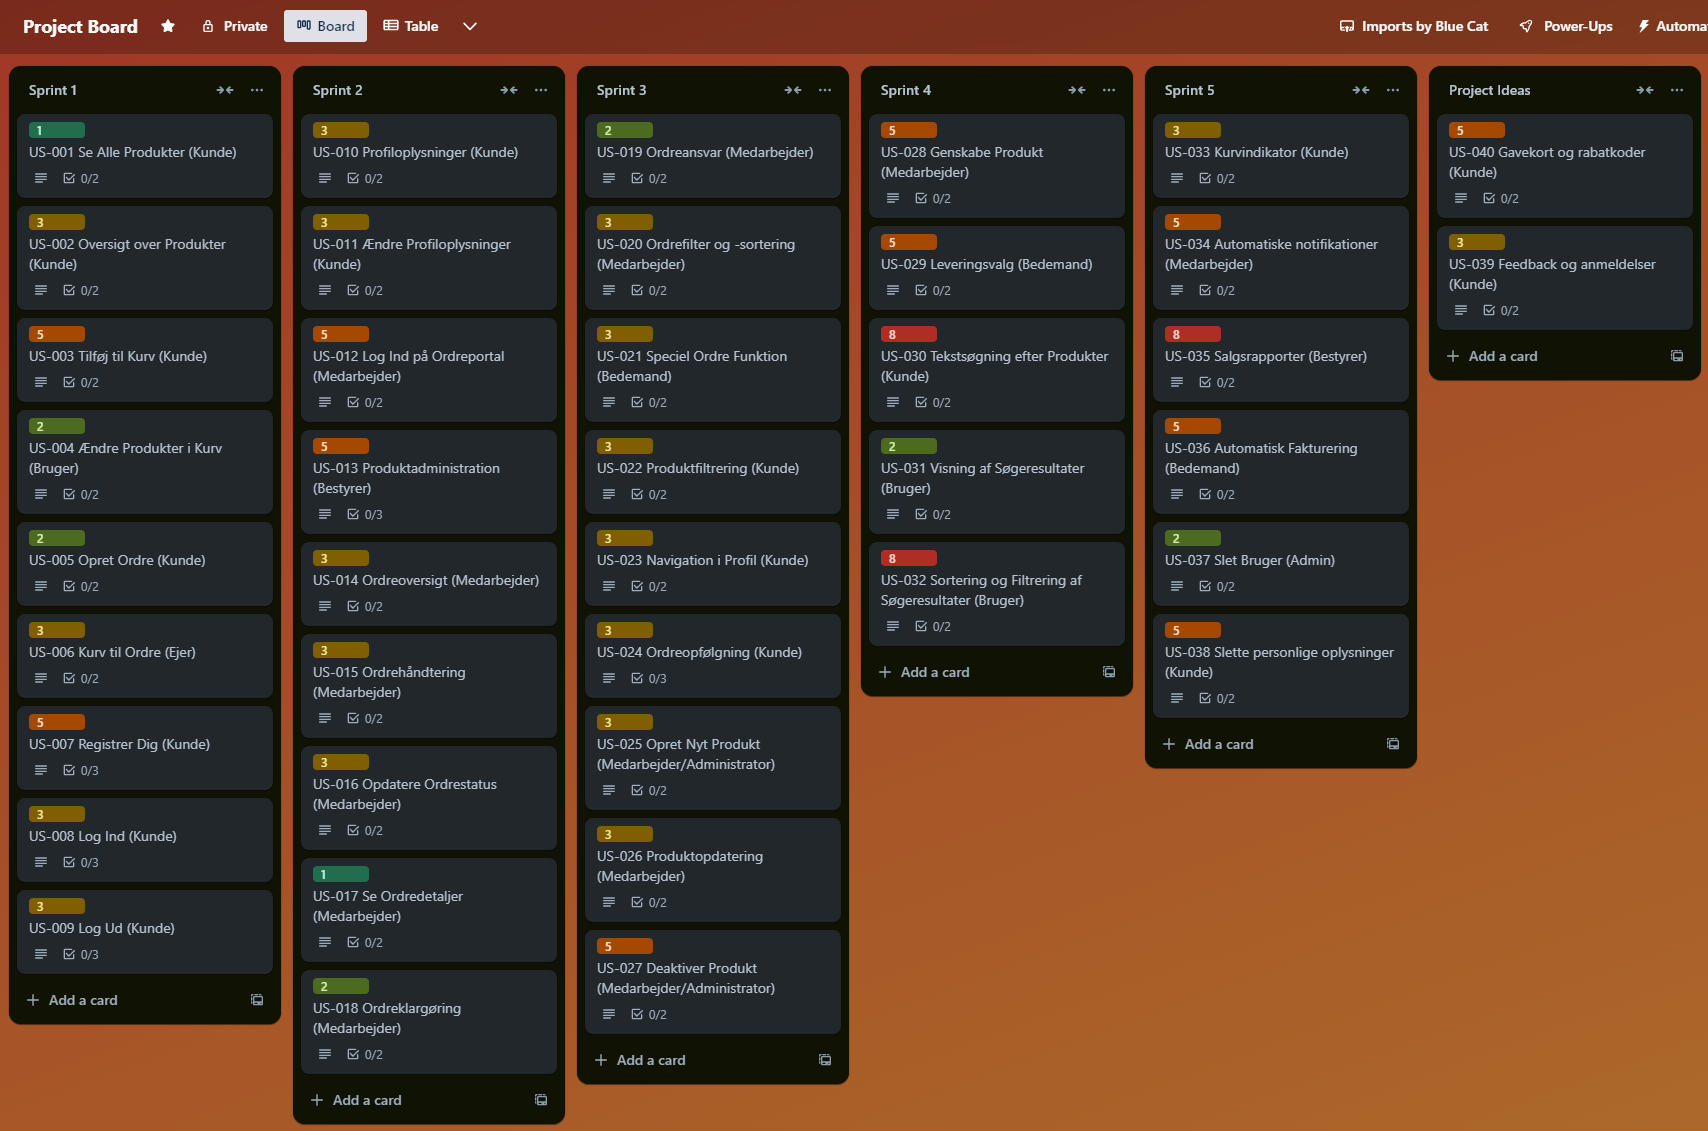
\includegraphics[width=0.9\textwidth]{figures/scrum/trello-sprint-backlogs.png}
    \caption{\emph{Product Backlog}}
    \label{fig:trello-sprint-backlogs}
\end{figure}

\section{Sprints}
\emph{Sprints} blev planlagt til at vare én uge, da det var en passende længde til at kunne implementere en vis mængde \emph{User Stories} (med tilhørende debugging, dokumentation etc.), men kort nok til at få en fornemmelse af \emph{velocity}.

\subsection{Sprint Planning}
\emph{Sprint Planning} blev en mere organisk, iterativ proces, med udgangspunkt i den første estimering og fordeling på \emph{Sprints}. 
Pointer fra \emph{Sprint Reviews} blev brugt til efterfølgende \emph{Sprint Planning}, så der blev taget højde for eventuelle forsinkelser eller overestimeringer.

\subsection{Daily Standup}
\emph{Daily Standup} blev mere til en daglig refleksion, da der kun var én udvikler. Da softwareudvikling ind imellem kræver den "gode idé" eller samtaler med ens gummiand, så blev der også taget højde for, om der skulle bruges kræfter andetsteds.
Der kunne stadig dokumenteres m.m. som ikke nødvendigvis var en del af den daglige udvikling.

\subsection{Sprint Review}
\emph{Sprint Review} blev brugt til at reflektere og evaluere, hvad der var blevet implementeret og hvad der manglede. Det blev også brugt til at justere \emph{Product Backloggen}, hvis der var \emph{User Stories}, der ikke længere var relevante eller \emph{User Stories}, der skulle tilføjes.
\emph{Burndown Chart} blev brugt til at visualisere og bestemme \emph{velocity} for \emph{Sprintet} og projektet som helhed.

\subsection{Sprint Retrospective}
\emph{Sprint Retrospective} var mere en selvransagelse end en gruppediskussion, da der kun var én udvikler. Der var dog stadig fokus på, hvad der var gået godt, og hvad der kunne forbedres. 
Bl.a. blev der reflekteret over, om der var \emph{User Stories}, der var over- eller underestimeret, og hvad der kunne gøres for at forbedre det. 
Et andet eksempel var, om der var blevet lagt en for stor indsats i en bestemt implementering og hvornår det gik fra, at ville finde en løsning til at ville "besejre" et problem.

\section{Burndown Chart}
\emph{Burndown Chart} blev brugt til at visualisere, hvor mange \emph{Story Points} der var tilbage i \emph{Sprintet} og projektet som helhed.

\section{Velocity}
\emph{Velocity} blev brugt til at estimere, hvor mange \emph{User Stories} der kunne implementeres i et \emph{Sprint}, og dermed hvor mange \emph{User Stories} der kunne implementeres i projektet som helhed.
\emph{Velocity} blev beregnet som gennemsnittet af de seneste \emph{Sprints}, da det gav et mere retvisende billede af, hvor mange \emph{Story Points} der kunne implementeres i et \emph{Sprint}.